\documentclass{article} % For LaTeX2e
\usepackage{nips14submit_e,times,xcolor}
\usepackage[colorlinks, citecolor={green!70!black}]{hyperref}
\usepackage{url}
\usepackage{amsmath,amssymb}
\usepackage{booktabs,multirow}
%\usepackage[backend=bibtex,
%            style=numeric,
%            firstinits=true,
%            natbib=true,
%            maxbibnames=20]{biblatex}
\usepackage{graphicx}
\usepackage{caption,subcaption}

%\usepackage{natbib} % EVB

\newtheorem{remark}{Remark}


\title{Extended and Unscented Gaussian Processes}


\author{
    Daniel M.~Steinberg \\
    NICTA \\ 
 \texttt{daniel.steinberg@nicta.com.au} 
%    Sydney, Australia\\
\And
Edwin V.~Bonilla \\
The University of New South Wales \\
 \texttt{e.bonilla@unsw.edu.au} 
}

% The \author macro works with any number of authors. There are two commands
% used to separate the names and addresses of multiple authors: \And and \AND.
%
% Using \And between authors leaves it to \LaTeX{} to determine where to break
% the lines. Using \AND forces a linebreak at that point. So, if \LaTeX{}
% puts 3 of 4 authors names on the first line, and the last on the second
% line, try using \AND instead of \And before the third author name.

\newcommand{\fix}{\marginpar{FIX}}
\newcommand{\new}{\marginpar{NEW}}
\renewcommand*{\sectionautorefname}{\S\!}
\renewcommand*{\subsectionautorefname}{\S\!}
%% Define bracket commands (normal, square and curly).
\newcommand{\brac} [1]  {\ensuremath{\left({#1}\right)}}
\newcommand{\sbrac}[1]  {\ensuremath{\left[{#1}\right]}}
\newcommand{\cbrac}[1]  {\ensuremath{\left\{{#1}\right\}}}
\newcommand{\abrac}[1]  {\ensuremath{\left\langle{#1}\right\rangle}}


%% Symbols

% General
\newcommand{\test}       {\ensuremath{^{*}}}
\newcommand{\testT}      {\ensuremath{^{*\top}\!}}
\newcommand{\ttest}      {\ensuremath{^{**}}}
\newcommand{\real}  [1] {\ensuremath{\mathbb{R}^{#1}}}
\newcommand{\ident} [1] {\ensuremath{\mathbf{I}_{#1}}}

% Variables
\newcommand{\lstate}    {\ensuremath{\mathbf{f}}}
\newcommand{\lcov}      {\ensuremath{\boldsymbol{\Sigma}}}
\newcommand{\obs}       {\ensuremath{\mathbf{y}}}
\newcommand{\hyper}     {\ensuremath{\boldsymbol{\theta}}}
\newcommand{\prmean}    {\ensuremath{\boldsymbol{\mu}}}
\newcommand{\prcov}     {\ensuremath{\mathbf{K}}}
\newcommand{\pomean}    {\ensuremath{\mathbf{m}}}
\newcommand{\pocov}     {\ensuremath{\mathbf{C}}}
\newcommand{\xcov}      {\ensuremath{\boldsymbol\Sigma_{\obs\pomean}}}
\newcommand{\Sobs}      {\ensuremath{\mathcal{Y}}}
\newcommand{\Sfunc}     {\ensuremath{\mathcal{M}}}
\newcommand{\scoef}     {\ensuremath{\kappa}}
\newcommand{\Sw}        {\ensuremath{w}}
\newcommand{\Kgain}     {\ensuremath{\mathbf{H}}}
\newcommand{\Linmat}    {\ensuremath{\mathbf{A}}}
\newcommand{\intcpt}    {\ensuremath{\mathbf{b}}}
\newcommand{\Fengy}     {\ensuremath{\mathcal{F}}}
\newcommand{\step}      {\ensuremath{\alpha}}
\newcommand{\jacob}[1]  {\ensuremath{\mathbf{J}_{#1}}}

% Augmented systems
\newcommand{\augobs}    {\ensuremath{\mathbf{z}}}
\newcommand{\augcov}    {\ensuremath{\mathbf{S}}}
\newcommand{\augLinmat} {\ensuremath{\mathbf{B}}}
\newcommand{\augintcpt} {\ensuremath{\mathbf{c}}}

% Gaussian Process
\newcommand{\obss}      {\ensuremath{y}}
\newcommand{\lstates}   {\ensuremath{f}}
\newcommand{\Lins}      {\ensuremath{a}}
\newcommand{\Linvec}    {\ensuremath{\mathbf{a}}}
\newcommand{\intcpts}   {\ensuremath{b}}
\newcommand{\inobs}     {\ensuremath{\mathbf{x}}}
\newcommand{\kernl}     {\ensuremath{k}}
\newcommand{\Kernl}     {\ensuremath{\mathbf{k}}}
\newcommand{\KERNL}     {\ensuremath{\mathbf{K}}}
\newcommand{\lvar}      {\ensuremath{\sigma^2}}
\newcommand{\lstd}      {\ensuremath{\sigma}}
\newcommand{\Lvar}      {\ensuremath{\boldsymbol\Lambda}}
\newcommand{\pomeans}   {\ensuremath{m}}
\newcommand{\pocovs}    {\ensuremath{C}}
\newcommand{\xcovs}     {\ensuremath{\Sigma}}
\newcommand{\khyper}    {\ensuremath{\theta}}
\newcommand{\khypers}   {\ensuremath{\boldsymbol\theta}}


%% Operations
\newcommand{\transpose}  {\ensuremath{^{\!\top}}}
\newcommand{\inv}        {\ensuremath{^{\text{-}1}}}
\newcommand{\deter}[1]   {\ensuremath{\left|{#1}\right|}}
\newcommand{\trace}[1]   {\ensuremath{\text{tr}\!\brac{#1}}}
\newcommand{\diag}[1]    {\ensuremath{\text{diag}\!\brac{#1}}}
\newcommand{\expec}[2]   {\ensuremath{\abrac{#2}_{#1}}}
\newcommand{\expece}[2]  {\ensuremath{\mathbb{E}_{#1}\!\sbrac{#2}}}
\newcommand{\evar} [2]   {\ensuremath{\mathbb{V}_{#1}\!\sbrac{#2}}}
\newcommand{\KL}[2]      {\ensuremath{\text{KL}\!\sbrac{{#1}\!\parallel\!{#2}}}}
\newcommand{\entropy}[1] {\ensuremath{\mathbb{H}\sbrac{#1}}}
\newcommand{\lnorm}[2]   {\ensuremath{\left\|{#2}\right\|_{{#1}}}}


%% Functions, PDFs etc
\newcommand{\nonlin}[1] {\ensuremath{g\!\brac{{#1}}}}
\newcommand{\augnonlin}[1] {\ensuremath{h\!\brac{{#1}}}}
\newcommand{\prob}  [1] {\ensuremath{p\!\brac{#1}}}
\newcommand{\probC} [2] {\ensuremath{p\!\left({#1}\middle\vert{#2}\right)}}
\newcommand{\qrob}  [1] {\ensuremath{q\!\brac{#1}}}
\newcommand{\qrobC} [2] {\ensuremath{q\!\left({#1}\middle\vert{#2}\right)}}
\newcommand{\gaus}  [1] {\ensuremath{\mathcal{N}\!\brac{#1}}}
\newcommand{\gausC} [2] {\ensuremath{\mathcal{N}\!\left({#1}\middle\vert{#2}\right)}}
\newcommand{\bern}  [1] {\ensuremath{\textrm{Bern}\!\brac{#1}}}
\newcommand{\bernC} [2] {\ensuremath{\textrm{Bern}\!\left({#1}\middle\vert{#2}\right)}}
\newcommand{\kfunc} [2] {\ensuremath{\kernl\!\brac{{#1}, {#2}}}}
\newcommand{\expon} [2] {\ensuremath{{#1}\!\times\!10^{#2}}}


%% Operators
\DeclareMathOperator*{\argmax}{\operatorname*{argmax}}
\DeclareMathOperator*{\argmin}{\operatorname*{argmin}}


\nipsfinalcopy % Uncomment for camera-ready version

\begin{document}


\maketitle

\begin{abstract}

    We present two new methods for inference in Gaussian process (GP) models
    with general nonlinear likelihoods. Inference is based on a variational
    framework where a Gaussian posterior is assumed and the likelihood is
    linearized about the variational posterior mean using either a %first order
    Taylor series expansion or statistical linearization. We show that the
    parameter updates obtained by these algorithms are equivalent to the state
    update equations in the iterative extended and unscented Kalman filters
    respectively, hence we refer to our algorithms as extended and unscented
    GPs. The unscented GP treats the likelihood as a `black-box' by not
    requiring its derivative for inference, so it also applies to
    non-differentiable likelihood models. We evaluate the performance of our
    algorithms on a  number of synthetic inversion problems and a binary
    classification dataset.
    
\end{abstract}


\section{Introduction}

Nonlinear inversion problems, where we wish to infer the latent inputs to a
system given observations of its output and the system's forward-model, have a
long history in the natural sciences, dynamical modeling and estimation. An
example is the robot-arm inverse kinematics problem. We wish to infer how to
drive the robot's joints (i.e.~joint torques) in order to place the
end-effector in a particular position, given we can measure its position and
know the forward kinematics of the arm. Most of the existing algorithms either
estimate the system inputs at a particular point in time like the
Levenberg-Marquardt algorithm \cite{Marquardt1963}, or in a recursive manner
such as the extended and unscented Kalman filters (EKF, UKF) \cite{Julier2004}. 

In many inversion problems we have a continuous process; a smooth trajectory of
a robot arm for example. Non-parametric regression techniques like Gaussian
processes \cite{Rasmussen2006} seem applicable, and have been used in linear
inversion problems \cite{Reid2013}. Similarly, Gaussian processes have been
used to learn inverse kinematics and predict the motion of a dynamical system
such as robot arms \cite{Rasmussen2006, Williams2008} and a human's gait
\cite{Lawrence2003, Wang2005, Wang2008}.  However, in \cite{Rasmussen2006,
    Williams2008} the inputs (torques) to the system are observable (not
latent) and are used to train the GPs. Whereas \cite{Wang2005, Wang2008} are
not concerned with inference over the original latent inputs, but rather they
want to find a low dimensional representation of high dimensional outputs for
prediction using Gaussian process latent variable models \cite{Lawrence2003}.
In this paper we introduce inference algorithms for GPs that can infer and
predict the original latent inputs to a system, without having to be explicitly
trained on them.

If we do not need to infer the latent inputs to a system it is desirable to
still incorporate domain/system specific information into an algorithm in terms
of a likelihood model specific to the task at hand. For example, non-parametric
classification or robust regression problems. In these situations it is useful
to have an inference procedure that does not require re-derivation for each new
likelihood model without having to resort to MCMC. An example of this is the
variational algorithm presented in \cite{Opper2009} for factorizing likelihood
models. In this model, the expectations arising from the use of arbitrary
(non-conjugate) likelihoods are only one-dimensional, and so they can be easily
evaluated using sampling techniques or quadrature. 
%
We present two alternatives to this algorithm that are also underpinned by
variational principles but are based on linearizing the nonlinear likelihood
models about the posterior mean. These methods are straight-forwardly
applicable to non-factorizing likelihoods and would retain computational
efficiency, unlike \cite{Opper2009} which would require evaluation of
multidimensional intractable integrals. One of our algorithms, based on
statistical linearization, does not even require derivatives of the likelihood
model (like \cite{Opper2009}) and so non-differentiable likelihoods can be
incorporated.

Initially we formulate our models in \autoref{sec:gausmod} for the
\emph{finite} Gaussian case because the linearization methods are more general
and comparable with existing algorithms. In fact we show we can derive the
update steps of the iterative EKF \cite{Bell1993} and similar updates to the
iterative UKF \cite{Sibley2006} using our variational inference procedures.
Then in \autoref{sec:gpmod} we specifically derive a factorizing likelihood
Gaussian process model using our framework, which we use for experiments in
\autoref{sec:experiments}.


\section{Variational Inference in Nonlinear Gaussian Models with Linearization}
\label{sec:gausmod}

Given some observable quantity $\obs \in \real{d}$, and a likelihood model for
the system of interest, in many situations it is desirable to reason about the
latent input to the system, $\lstate\in\real{D}$, that generated the
observations. Finding these inputs is an inversion problem and in a
probabilistic setting it can be cast as an application of Bayes' rule.
%\begin{equation}
 %   \probC{\lstate}{\obs} = \frac{\probC{\obs}{\lstate}\prob{\lstate}}
 %       {\prob{\obs}}.
%    \label{eq:bayesrule}
%\end{equation}
The following forms are assumed for the prior and likelihood:
\begin{equation}
    \prob{\lstate} = \gausC{\lstate}{\prmean, \prcov}
    \quad \text{and} \quad
    \probC{\obs}{\lstate} = \gausC{\obs}{\nonlin{\lstate}, \lcov},
    \label{eq:priorlike}
\end{equation}
where $\nonlin{\cdot} : \real{D} \to \real{d}$ is a nonlinear function or
forward model. Unfortunately the marginal likelihood, $\prob{\obs}$, is
intractable as the nonlinear function makes the likelihood and prior
non-conjugate.
%\begin{equation}
%    \prob{\obs} = \int \gausC{\obs}{\nonlin{\lstate}, \lcov}
%        \gausC{\lstate}{\prmean, \prcov} d\lstate,
%    \label{eq:marglike}
%\end{equation}
This also makes the posterior $\probC{\lstate}{\obs}$, which is the solution to
the inverse problem, intractable to evaluate.  So, we choose to approximate the
posterior with variational inference \cite{Jordan1999}.


\subsection{Variational Approximation}

Using variational inference procedures we can put a lower bound on the
log-marginal likelihood using Jensen's inequality, 
\begin{equation}
    \log \prob{\obs} \geq \int \qrob{\lstate} \log 
        \frac{\probC{\obs}{\lstate}\prob{\lstate}}{\qrob{\lstate}} d\lstate,
\end{equation}
with equality iff $\KL{\qrob{\lstate}}{\probC{\lstate}{\obs}} = 0$, and where
$\qrob{\lstate}$ is an approximation to the true posterior,
\probC{\lstate}{\obs}. This lower bound is often referred to as `free energy',
and can be re-written as follows
\begin{equation}
    \Fengy = \expec{q\lstate}{\log \probC{\obs}{\lstate}}
        - \KL{\qrob{\lstate}}{\prob{\lstate}},
    \label{eq:fengy}
\end{equation}
where $\expec{q\lstate}{\cdot}$ is an expectation with respect to the
variational posterior, $\qrob{\lstate}$. We assume the posterior takes a
Gaussian form, $\qrob{\lstate} = \gausC{\lstate}{\pomean, \pocov}$, so
we can evaluate the expectation and KL term in~\eqref{eq:fengy},
\begin{align}
    \expec{q\lstate}{\log \probC{\obs}{\lstate}}
        =& -\frac{1}{2} \bigg[ 
            D\log{2\pi} + \log\deter{\lcov} 
            + \expec{q\lstate}{\brac{\obs - \nonlin{\lstate}}\transpose\lcov\inv
            \brac{\obs - \nonlin{\lstate}}}\bigg],
            \label{eq:qlike} \\
     \KL{\qrob{\lstate}}{\prob{\lstate}}
        =& ~\frac{1}{2} \bigg[\trace{\prcov\inv\pocov}
        + \brac{\prmean - \pomean}\transpose\prcov\inv
        \brac{\prmean - \pomean} 
        - \log\deter{\pocov} + \log\deter{\prcov}
        - D\bigg] \label{eq:qkl}.
\end{align}
where the expectation involving $\nonlin{\cdot}$ may be intractable. One method
of dealing with these expectations is presented in \cite{Opper2009} by assuming
that the likelihood factorizes across observations. Here we provide two
alternatives based on linearizing $\nonlin{\cdot}$ about  the posterior mean,
$\pomean$.


\subsection{Parameter Updates}

To find the optimal posterior mean, $\pomean$, we need to find the derivative,
\begin{equation}
    \frac{\partial\Fengy}{\partial\pomean} = -\frac{1}{2}
    \frac{\partial}{\partial\pomean} \expec{q\lstate}{
        \brac{\prmean - \lstate}\transpose\prcov\inv
        \brac{\prmean - \lstate}
        + \brac{\obs - \nonlin{\lstate}}\transpose \lcov\inv
            \brac{\obs - \nonlin{\lstate}}},
\end{equation}
where all terms in $\Fengy$ independent of $\pomean$ have been dropped, and we
have placed the quadratic and trace terms from the KL component in Equation
\eqref{eq:qkl} back into the expectation.
We can represent this as an augmented Gaussian,
\begin{equation}
    \frac{\partial\Fengy}{\partial\pomean} = -\frac{1}{2}
        \frac{\partial}{\partial\pomean}
        \expec{q\lstate}{
        \brac{\augobs - \augnonlin{\lstate}}\transpose\augcov\inv
        \brac{\augobs - \augnonlin{\lstate}}
    },
    \label{eq:augsys}
\end{equation}
where
\begin{equation}
    \augobs = \begin{bmatrix} \obs \\ \prmean \end{bmatrix}, \quad
    \augnonlin{\lstate} = \begin{bmatrix} \nonlin{\lstate} \\ \lstate 
        \end{bmatrix}, \quad
    \augcov = \begin{bmatrix} \lcov & \mathbf{0} \\ \mathbf{0} & \prcov 
        \end{bmatrix}.
\end{equation}
Now we can see solving for $\pomean$ is essentially a nonlinear least squares 
problem%
    %\footnote{$-\frac{1}{2}
        %\frac{\partial}{\partial\lstate}
        %\brac{\augobs - \augnonlin{\lstate}}\transpose\augcov\inv
        %\brac{\augobs - \augnonlin{\lstate}} = 0$.}
, but about
the expected posterior value of $\lstate$. Even without the expectation, there
is no  closed form solution to $\partial\Fengy/\partial\pomean = 0$.
However, we can use an iterative Newton method to find $\pomean$. It begins
with an initial guess, $\pomean_0$, then proceeds with the iterations,
\begin{equation}
    \pomean_{k+1} = \pomean_k -
    \step\brac{\nabla_\pomean\nabla_\pomean\Fengy}\inv \nabla_\pomean\Fengy,
    \label{eq:newton}
\end{equation}
for some step length, $\step \in (0, 1]$. Though evaluating
$\nabla_\pomean\Fengy$ is still intractable because of the nonlinear term
within the expectation in Equation \eqref{eq:augsys}. If we linearize
$\nonlin{\lstate}$, we can evaluate the expectation,
\begin{equation}
    \nonlin{\lstate} \approx \Linmat\lstate + \intcpt,
    \label{eq:linearize}
\end{equation}
for some linearization matrix $\Linmat \in \real{d \times D}$ and an intercept
term $\intcpt \in \real{d}$. Using this we get,
\begin{equation}
    \nabla_\pomean \Fengy
        \approx \Linmat\transpose\lcov\inv\brac{\obs - \Linmat\pomean 
            - \intcpt} + \prcov\inv\brac{\prmean - \pomean}
    \quad \text{and} \quad
    \nabla_\pomean \nabla_\pomean \Fengy
        \approx - \prcov\inv - \Linmat\transpose\lcov\inv\Linmat.
        \label{eq:deldelF}
\end{equation}
Substituting \eqref{eq:deldelF} into \eqref{eq:newton} and using the Woodbury
identity we can derive the iterations,
\begin{equation}
    \pomean_{k+1} = \brac{1-\step}\pomean_k + \step\prmean 
        + \step\Kgain_k\brac{\obs - \intcpt_k - \Linmat_k\prmean},
    \label{eq:pomean}
\end{equation}
where $\Kgain_k$ is usually referred to as  a ``Kalman gain'' term,
\begin{equation}
    \Kgain_k = \prcov\Linmat_k\transpose\brac{\lcov +
        \Linmat_k\prcov\Linmat_k\transpose}\inv,
    \label{eq:kgain}
\end{equation}
and we have assumed that the linearization $\Linmat_k$ and intercept,
$\intcpt_k$ are in some way dependent on the iteration. We can find the 
posterior covariance by setting $\partial\Fengy/\partial\pocov = 0$ where,
\begin{equation}
    \frac{\partial\Fengy}{\partial\pocov} = -\frac{1}{2} 
        \frac{\partial}{\partial\pocov}
        \expec{q\lstate}{
            \brac{\augobs - \augnonlin{\lstate}}\transpose\augcov\inv
            \brac{\augobs - \augnonlin{\lstate}}
    } 
    + \frac{1}{2} \frac{\partial}{\partial\pocov} \log \deter{\pocov}.
\end{equation}
Again we do not have an analytic solution, so we once more apply the
approximation \eqref{eq:linearize} to get,
\begin{equation}
    \pocov = \sbrac{\prcov\inv + \Linmat\transpose\lcov\inv\Linmat}\inv
        %\approx - \brac{\nabla_\pomean \nabla_\pomean \Fengy}\inv.
    = \brac{\ident{D} - \Kgain\Linmat}\!\prcov,
    \label{eq:pocov}
\end{equation}
%Using the Woodbury identity,
%\begin{equation}
    %\pocov = \brac{\ident{D} - \Kgain\Linmat}\!\prcov
    %\label{eq:pocov}
%\end{equation}
where we have once more made use of the Woodbury identity and also the
\emph{converged} values of $\Linmat$ and $\Kgain$. At this point it is also
worth noting the relationship between Equations \eqref{eq:pocov} and
\eqref{eq:deldelF}.


\subsection{Taylor Series Linearization}

Now we need to find expressions for the linearization terms $\Linmat$ and
$\intcpt$. One method is to use a first order Taylor Series expansion to 
linearize $\nonlin{\cdot}$ about the last calculation of the posterior mean, 
$\pomean_k$,
\begin{equation}
    \nonlin{\lstate} \approx \nonlin{\pomean_k} +
    \jacob{\pomean_k}\brac{\lstate - \pomean_k},
\end{equation}
where $\jacob{\pomean_k}$ is the Jacobian $\partial\nonlin{\pomean_k}\!/
\partial\pomean_k$. By linearizing the function in this way we end up with a
\emph{Gauss-Newton} optimization procedure for finding $\pomean$. Equating
coefficients with \eqref{eq:linearize}, 
\begin{equation}
    \Linmat = \jacob{\pomean_k}, \qquad \intcpt = \nonlin{\pomean_k} -
    \jacob{\pomean_k}\pomean_k,
\end{equation}
and then substituting these values into Equations
\eqref{eq:pomean} -- \eqref{eq:pocov} we get,
\begin{align}
    \pomean_{k+1} &= \brac{1-\step}\pomean_k + \step\prmean 
        + \step\Kgain_k\brac{\obs - \nonlin{\pomean_k} 
        + \jacob{\pomean_k}\brac{\pomean_k - \prmean}},
    \label{eq:pomean_ekf} \\
    \Kgain_k &= \prcov\jacob{\pomean_k}\transpose\brac{\lcov +
        \jacob{\pomean_k}\prcov\jacob{\pomean_k}\transpose}\inv, \\
    \pocov &= \brac{\ident{D} - \Kgain\jacob{\pomean}}\!\prcov.
    \label{eq:pocov_ekf}
\end{align}
Here $\jacob{\pomean}$ and $\Kgain$ without the $k$ subscript are constructed
about the converged posterior, $\pomean$. 
%
\begin{remark}
A single step of the  iterated extended Kalman filter~\cite{Bell1993,
    Sibley2006} corresponds to an update  in our variational framework when
using the Taylor series linearization of the non-linear forward model
$g(\cdot)$ around the posterior mean.
\end{remark}
Having derived the updates in our variational framework, the proof of this is
trivial by making  $\step =1$, and using Equations \eqref{eq:pomean_ekf} --
\eqref{eq:pocov_ekf} as the iterative updates.


\subsection{Statistical Linearization}

Another method for linearizing $\nonlin{\cdot}$ is \emph{statistical
    linearization} (see e.g.~\cite{Geist2010}), which finds a least squares
best fit to $\nonlin{\cdot}$ about a point. The advantage of this method is
that it does not require derivatives
$\partial\nonlin{\lstate}\!/\partial\lstate$. To obtain the fit, multiple
observations of the forward model $\nonlin{\cdot}$ at different input points
are required. Hence, the key question is where to evaluate our forward model so
as to obtain representative samples to carry out the linearization.  One method
of obtaining these points is the unscented transform \cite{Julier2004}, which
defines $2D+1$ `sigma' points,
\begin{align}
    \Sfunc_0 &= \pomean,
        \label{eq:spoint0} \\
    \Sfunc_i &= \pomean + \brac{\sqrt{\brac{D + \scoef} \pocov}}_i \quad
        \text{for} \quad i = 1 \ldots D, \\
    \Sfunc_i &= \pomean - \brac{\sqrt{\brac{D + \scoef} \pocov}}_i \quad
        \text{for} \quad i = D+1 \ldots 2D,
        \label{eq:spointi} \\
    \Sobs_i &= \nonlin{\Sfunc_i} \text{,}
\end{align}
for a free parameter $\scoef$. 
Here $(\sqrt{\cdot})_i$ refers to columns of the matrix square root, we follow
\cite{Julier2004} and use the Cholesky decomposition. Unlike the usual
unscented transform, which uses the prior to create the sigma points, here we
have used the posterior because of the expectation in \eqref{eq:augsys}. Using
these points we can define the following statistics,
\begin{alignat}{2}
    \bar\obs &= \sum^{2D}_{i=0} \Sw_i \Sobs_i,
    \qquad
    &\xcov = \sum^{2D}_{i=0} \Sw_i \brac{\Sobs_i - \bar\obs}
        \brac{\Sfunc_i - \pomean}\transpose,
    \label{eq:slstats} \\
    \Sw_0 &= \frac{\scoef}{D + \scoef},
        &\Sw_i = \frac{1}{2\brac{D + \scoef}}
        \quad \text{for} \quad i = 1 \ldots 2D \text{.}
    \label{eq:slweights}
\end{alignat}
According to \cite{Julier2004} various settings
of $\scoef$ can capture information about the higher order moments of the
distribution of $\obs$; or setting $\scoef = 0.5$ yields uniform weights.
Therefore, the objective of statistical linearization is,
\begin{equation}
    \argmin_{\Linmat, \intcpt} \sum^{2D}_{i=0} 
        \lnorm{2}{\Sobs_i - \brac{\Linmat\Sfunc_i + \intcpt}}^2.
\end{equation}
This is simply linear least-squares and has the solution \cite{Geist2010}:
\begin{equation}
    \Linmat = \xcov \pocov\inv, \qquad
    \intcpt = \bar\obs - \Linmat\pomean.
\end{equation}
Substituting $\intcpt$ back into Equation \eqref{eq:pomean}, we obtain, 
\begin{equation}
    \pomean_{k+1} = \brac{1-\step}\pomean_k + \step\prmean 
        + \step\Kgain_k\brac{\obs - \bar\obs_k 
        + \Linmat_k\brac{\pomean_k - \prmean}}.
    \label{eq:pomean_sl}
\end{equation}

Here $\Kgain_k$, $\Linmat_k$ and $\bar\obs_k$ have been evaluated using the
statistics from the $k$th iteration. This implies that the posterior
covariance, $\pocov_k$, is now estimated at every iteration of
\eqref{eq:pomean_sl} since we use it to form $\Linmat_k$ and $\intcpt_k$.
$\Kgain_k$ and $\pocov_k$ have the same form as Equations \eqref{eq:kgain} and
\eqref{eq:pocov} respectively. 

\begin{remark}
A single step of the  iterated unscented sigma-point Kalman filter (iSPKF,
\cite{Sibley2006}) can be seen as an ad hoc approximation to an update in our
statistically linearized variational framework. 
\end{remark}

Equations \eqref{eq:pomean_sl} and \eqref{eq:pocov} are equivalent to the
equations for a single update of the iterated sigma-point Kalman filter (iSPKF)
for $\step = 1$, except for the term $\bar\obs_k$ appearing in Equation
\eqref{eq:pomean_sl} as opposed to $\nonlin{\pomean_k}$. The main difference is
that we have derived our updates from variational principles.
%Furthermore, we
%have found experimentally that the updates in Equations \eqref{eq:pomean_sl}
%and \eqref{eq:pocov} provide better results consistently across a wide variety
%of problems.
%
These updates are also more similar to the regular recursive unscented Kalman
filter \cite{Julier2004}, and statistically linearized recursive least squares
\cite{Geist2010}.


\subsection{Optimizing the Posterior}

Because of the expectations involving an arbitrary function in Equation
\eqref{eq:qlike}, no analytical solution exists for the lower bound on the
marginal likelihood, $\Fengy$. We can use our approximation
\eqref{eq:linearize} again,
\begin{multline}
    \Fengy \approx - \frac{1}{2} \bigg[
    D\log{2\pi} + \log\deter{\lcov} - \log\deter{\pocov} + \log{\deter{\prcov}}
    + \brac{\prmean - \pomean}\transpose\prcov\inv
    \brac{\prmean - \pomean} \\
    + \brac{\obs - \Linmat\pomean - \intcpt}\transpose\lcov\inv
        \brac{\obs - \Linmat\pomean - \intcpt}
        \bigg].
    \label{eq:approxfengy}
\end{multline}
Here the trace term from Equation \eqref{eq:qkl} has cancelled with a trace
term from the expected likelihood,
$\trace{\Linmat\transpose\lcov\inv\Linmat\pocov} = D -
\trace{\prcov\inv\pocov}$ once we have linearized $\nonlin{\cdot}$ and
substituted \eqref{eq:pocov}. Unfortunately this approximation is no longer a
lower bound on the log marginal likelihood in general. In practice we only
calculate this approximation $\Fengy$ if we need to optimize some model
hyperparameters, like for a Gaussian process as described in
\autoref{sec:gpmod}. When optimizing $\pomean$, the only terms of $\Fengy$
dependent on $\pomean$ in the Taylor series linearization case are,
\begin{equation}
    -\frac{1}{2} \brac{\obs - \nonlin{\pomean}}\transpose
            \lcov\inv
            \brac{\obs - \nonlin{\pomean}} \\
    -\frac{1}{2}
    \brac{\prmean - \pomean}\transpose\prcov\inv\brac{\prmean - \pomean}.
    \label{eq:MAP}
\end{equation}
This is also the \emph{maximum a-posteriori} objective. A global convergence
proof exists for this objective when optimized by a Gauss-Newton procedure
under some conditions on the Jacobians, see \cite[p255]{Nocedal2006}.  No such
guarantees exist for statistical linearization, though monitoring
\eqref{eq:MAP} works well in practice (see the experiment in
\autoref{sec:exptoy}). 
A line search could be used to select an optimal value for the step length,
$\step$ in Equation \eqref{eq:pomean}. However, we find that setting $\step=1$,
and then successively multiplying $\step$ by some number in $\brac{0, 1}$ until
the MAP objective \eqref{eq:MAP} decreases, or some maximum number of
iterations is exceeded is fast and works well in practice. If the maximum
number of iterations is exceeded we call this a `diverge' condition, and
terminate the search for $\pomean$ (and return the last good value). This only
tends to happen for statistical linearization, but does not tend to impact the
algorithms performance since we always make sure to improve (approximate)
$\Fengy$.

\section{Variational Inference in Gaussian Process Models with Linearization}
\label{sec:gpmod}

We now present two inference methods for Gaussian Process (GP) models
\cite{Rasmussen2006} with arbitrary nonlinear likelihoods using the framework
presented previously.  Both Gaussian process models have the following
likelihood and prior,
\begin{equation}
    \obs \sim \gaus{\nonlin{\lstate}, \lvar\ident{N}}, \qquad
    \lstate \sim \gaus{\mathbf{0}, \KERNL}.
    \label{eq:gplikeprior}
\end{equation}
Here $\obs \in \real{N}$ are the $N$ noisy observed values of the transformed
latent function, $\nonlin{\lstate}$, and $\lstate \in \real{N}$ is the latent
function we are interested in inferring. $\KERNL \in \real{N\times N}$ is the
kernel matrix, where each element $\kernl_{ij} = \kernl\!\brac{\inobs_i,
    \inobs_j}$ is the result of applying a kernel function to each input,
$\inobs \in \real{P}$, in a pair-wise manner. It is also important to note that
the likelihood noise model is \emph{isotropic} with a variance of $\lvar$. This
is not a necessary condition, and we can use a correlated noise likelihood
model, however the factorized likelihood case is still useful and provides some
computational benefits. 
    
As before, we make the approximation that the posterior is Gaussian,
$\qrobC{\lstate}{\pomean, \pocov} = \gausC{\lstate}{\pomean, \pocov}$ where
$\pomean \in \real{N}$ is the mean posterior latent function, and $\pocov \in
\real{N \times N}$ is the posterior covariance. Since the likelihood is
isotropic and factorizes over the $N$  observations 
we have the following expectation under
our variational inference framework:
\begin{equation*}
    \expec{q\lstate}{\log\probC{\obs}{\lstate}} =
        - \frac{N}{2}\log{2\pi\lvar}
        - \frac{1}{2\lvar} \sum_{n=1}^N 
            \expec{q\lstates_n}{\brac{\obss_n - \nonlin{\lstates_n}}^2}.
\end{equation*}
As a consequence the linearization is one-dimensional, that is
$\nonlin{\lstates_n} \approx \Lins_n\lstates_n + \intcpts_n$.  Using this we
can derive the approximate gradients,
\begin{equation}
    \nabla_\pomean\Fengy \approx \frac{1}{\lvar}\Linmat\brac{\obs -
        \Linmat\pomean - \intcpt} - \KERNL\inv\pomean,
    \qquad
    \nabla_\pomean\nabla_\pomean \Fengy \approx -\KERNL\inv
    -\Linmat\Lvar\inv\Linmat,
\end{equation}
where $\Linmat = \diag{\sbrac{\Lins_1, \ldots, \Lins_N}}$ and $\Lvar =
\diag{\sbrac{\lvar, \ldots, \lvar}}$. Because of the factorizing likelihood we
obtain $\pocov\inv = \KERNL\inv + \Linmat\Lvar\inv\Linmat$, that is, the
inverse posterior covariance is just the prior inverse covariance, but with a
modified diagonal. This means if we were to use this inverse parameterization
of the Gaussian, which is also used in \cite{Opper2009}, we would only have to
infer $2N$ parameters (instead of $N + N(N+1)/2$). We can obtain the iterative
steps for $\pomean$ straightforwardly:
\begin{equation}
    \pomean_{k+1} = \brac{1-\step}\pomean_k 
        + \step\Kgain_k\brac{\obs - \intcpt_k}, 
        \quad \text{where} \quad
    \Kgain_k = \KERNL\Linmat_k\brac{\Lvar + \Linmat_k\KERNL\Linmat_k}\inv,
    \label{eq:pomeangp}
\end{equation}
and also for the posterior covariance,
\begin{equation}
    \pocov = \brac{\ident{N} - \Kgain\Linmat}\!\KERNL.
    \label{eq:pocovgp}
\end{equation}
The values for $\Lins_n$ and $\intcpts_n$ for the linearization methods are,
\begin{alignat}{3}
    \text{Taylor}:&\quad
        \Lins_n &= \frac{\partial\nonlin{\pomeans_n}}{\partial\pomeans_n},
        \quad
        \intcpts_n &= \nonlin{\pomeans_n}
        - \frac{\partial\nonlin{\pomeans_n}}{\partial\pomeans_n} \pomeans_n, \\
    \text{Statistical}:&\quad
        \Lins_n &= \frac{\xcovs_{\pomeans\obss,n}}{\pocovs_{nn}},
        \quad
        \intcpts_n &= \bar\obss_n - \Lins_n\pomeans_n.
\end{alignat}
$\pocovs_{nn}$ is the $n$th diagonal element of $\pocov$ and
$\xcovs_{\pomeans\obss,n}$ and $\bar\obss_n$ are scalar versions of Equations
\eqref{eq:spoint0} -- \eqref{eq:slweights} where the sigma points for each
observation, $n$, are $\Sfunc_{n} = \big\{\pomeans_n,~\pomeans_n +
\sqrt{\brac{1 + \scoef}\pocovs_{nn}},~\pomeans_n - \sqrt{\brac{1 +
        \scoef}\pocovs_{nn}}\big\}$. We refer to the Taylor series linearized
GP as the \emph{extended} GP (EGP), and the statistically linearized GP as the
\emph{unscented} GP (UGP). 


\subsection{Prediction}

To find the distribution for a test point, $\lstates\test$, 
we only need to combine our approximate Gaussian posterior with 
our GP prior. This
gives $\lstates\test \sim \gaus{\pomeans\test, \pocovs\test}$ where,
\begin{equation}
    \pomeans\test = \Kernl\testT\KERNL\inv\pomean,
    \qquad
    \pocovs\test = \kernl\ttest - \Kernl\testT\KERNL\inv\sbrac{\ident{N} -
        \pocov\KERNL\inv}\Kernl\test,
\end{equation}
and $\kernl\ttest = \kernl\!\brac{\inobs\test, \inobs\test}$ and $\Kernl\test
= \sbrac{\kernl\!\brac{\inobs_1, \inobs\test}, \ldots, \kernl\!\brac{\inobs_N,
        \inobs\test}}\transpose$. We can also find the predicted observations,
$\bar\obss\test$ by evaluating the one-dimensional integral,
\begin{equation}
    \bar\obss\test = \expec{q\lstates\test}{\obss\test} = \int
        \nonlin{\lstates\test} \gausC{\lstates\test}{\pomeans\test,
            \pocovs\test} d\lstates\test,
\end{equation}
for which we use quadrature.
%(specifically the scipy.integrate.quad routine\cite{JonesScipy}). 
Alternatively, if we were to use the UGP we can use another
application of the unscented transform to approximate the predictive
distribution $\obss\test \sim \gaus{\bar\obss\test, \lvar_{\obss\test}}$ where,
\begin{equation}
    \bar\obss\test = \sum^2_{i=0} \Sw_i \Sfunc_i\test, \qquad 
    \lvar_{\obss\test} = \sum^2_{i=0} \Sw_i \brac{\Sobs_i\test -
        \bar\obss\test}^2.
    \label{eq:slpred}
\end{equation}
This works well in practice, see \autoref{fig:learnex} for a demonstration.


\subsection{Learning the Linearized GPs}

Learning the extended and unscented GPs consists of  an inner and outer loop.
Much like the Laplace approximation for binary Gaussian Process classifiers
\cite{Rasmussen2006}, the inner loop is for learning the posterior mean,
$\pomean$, and the outer loop is to optimize the likelihood parameters
(e.g.~the variance $\lvar$) and kernel hyperparameters,
$\kfunc{\cdot}{\cdot|\khypers}$. The dominant computational cost in learning
the parameters is the inversion in Equation \eqref{eq:pomeangp}, and so the
computational complexity of the EGP and UGP is about the same as for the
Laplace GP approximation.
%
To learn the kernel hyperparameters and $\lvar$ we use numerical techniques
to find the gradients, $\partial\Fengy/\partial\khypers$, for both the
algorithms, where $\Fengy$ is approximated,
\begin{equation}
    \Fengy \approx - \frac{1}{2} \left[
    N\!\log{2\pi\lvar}
    %- \log\deter{\pocov\KERNL\inv}
    - \log\deter{\pocov}
    + \log\deter{\KERNL}
    + \pomean\transpose\KERNL\inv \pomean
    + \frac{1}{\lvar}
        \brac{\obs - \Linmat\pomean - \intcpt}\transpose\!
        \brac{\obs - \Linmat\pomean - \intcpt}
    \right].
    \label{eq:fengygp}
\end{equation}
Specifically we use derivative-free optimization methods (e.g. BOBYQA) from
the NLopt library~\cite{JohnsonNLOPT}, which we find fast and effective. This
also has the advantage of not requiring knowledge of
$\partial\nonlin{\lstates}\!/\partial\lstates$ or higher order derivatives for
any implicit gradient dependencies between $\lstate$ and~$\khypers$. 


\section{Experiments}
\label{sec:experiments}
%
%In this section we evaluate the performance of the EGP and UGP on a 
%set of synthetic inversion problems and on the USPS handwritten digits binary 
%classification problem.
%
%We have implemented both the EGP and UGP, as well as regular GP in python code
%using NLopt~\cite{JohnsonNLOPT} for hyperparameter learning (BOBYQA) and scipy
%\cite{JonesScipy} (scipy.integrate.quad) for quadrature.
%
%
\subsection{Toy Inversion Problems}
\label{sec:exptoy}

\begin{table}[tb]
    \centering
    \caption[]{The negative log predictive density (NLPD) and the standardized
        mean squared error (SMSE) on test data for various differentiable
        forward models. Lower values are better for both measures.  The predicted
        $\lstates\test$ and $\obss\test$ are the same for $\nonlin{\lstate} =
        \lstate$, so we do not report $\obss\test$ in this case.}

    \footnotesize
    \begin{tabular}{r|c| c c c c c c}
        \multirow{2}{*}{$\nonlin{\lstate}$} & \multirow{2}{*}{Algorithm} & 
            \multicolumn{2}{c}{NLPD $\lstates\test$} &
            \multicolumn{2}{c}{SMSE $\lstates\test$} &
            \multicolumn{2}{c}{SMSE $\obss\test$} \\
        & & mean & std. & mean & std. & mean & std.\\
        \toprule
        $\lstate$ 
& UGP & -0.90046 & 0.06743 & 0.01219 & 0.00171 & -- & -- \\
& EGP & -0.89908 & 0.06608 & 0.01224 & 0.00178 & -- & -- \\
& \cite{Opper2009} & -0.27590 & 0.06884 & 0.01249 & 0.00159 & -- & -- \\
& GP & -\textbf{0.90278} & 0.06988 & \textbf{0.01211} & 0.00160 & -- & -- \\
        \midrule
        $\lstate^3 + \lstate^2 + \lstate$ 
& UGP & -\textbf{0.23622} & 1.72609 & 0.01534 & 0.00202 &
\textbf{0.02184} & 0.00525 \\
& EGP & -0.22325 & 1.76231 & \textbf{0.01518} & 0.00203 & \textbf{0.02184} & 0.00528 \\
& \cite{Opper2009} & -0.14559 & 0.04026 & 0.06733 & 0.01421 & 0.02686 & 0.00266 \\
        \midrule
        $\exp\!\brac{\lstate}$ 
& UGP & -0.75475 & 0.32376 & \textbf{0.13860} & 0.04833 & \textbf{0.03865} & 0.00403 \\
& EGP & -\textbf{0.75706} & 0.32051 & 0.13971 & 0.04842 & 0.03872 & 0.00411 \\
& \cite{Opper2009} & -0.08176 & 0.10986 & 0.17614 & 0.04845 & 0.05956 & 0.01070 \\
        \midrule
        $\sin\!\brac{\lstate}$ 
& UGP & -\textbf{0.59710} & 0.22861 & \textbf{0.03305} & 0.00840 & 0.11513 & 0.00521 \\
& EGP & -0.59705 & 0.21611 & 0.03480 & 0.00791 & \textbf{0.11478} & 0.00532 \\
& \cite{Opper2009} & -0.04363 & 0.03883 & 0.05913 & 0.01079 & 0.11890 & 0.00652 \\
        \midrule
        $\tanh\!\brac{2\lstate}$
& UGP & \textbf{0.01101} & 0.60256 & \textbf{0.15703} & 0.06077 &
\textbf{0.08767} & 0.00292 \\
& EGP & 0.57403 & 1.25248 & 0.18739 & 0.07869 & 0.08874 & 0.00394 \\
& \cite{Opper2009} & 0.15743 & 0.14663 & 0.16049 & 0.04563 & 0.09434 & 0.00425 \\
        \bottomrule
    \end{tabular}
    \label{tab:toy}
\end{table}
%
\begin{figure}[tb]
    \begin{subfigure}[b]{0.5\linewidth}
        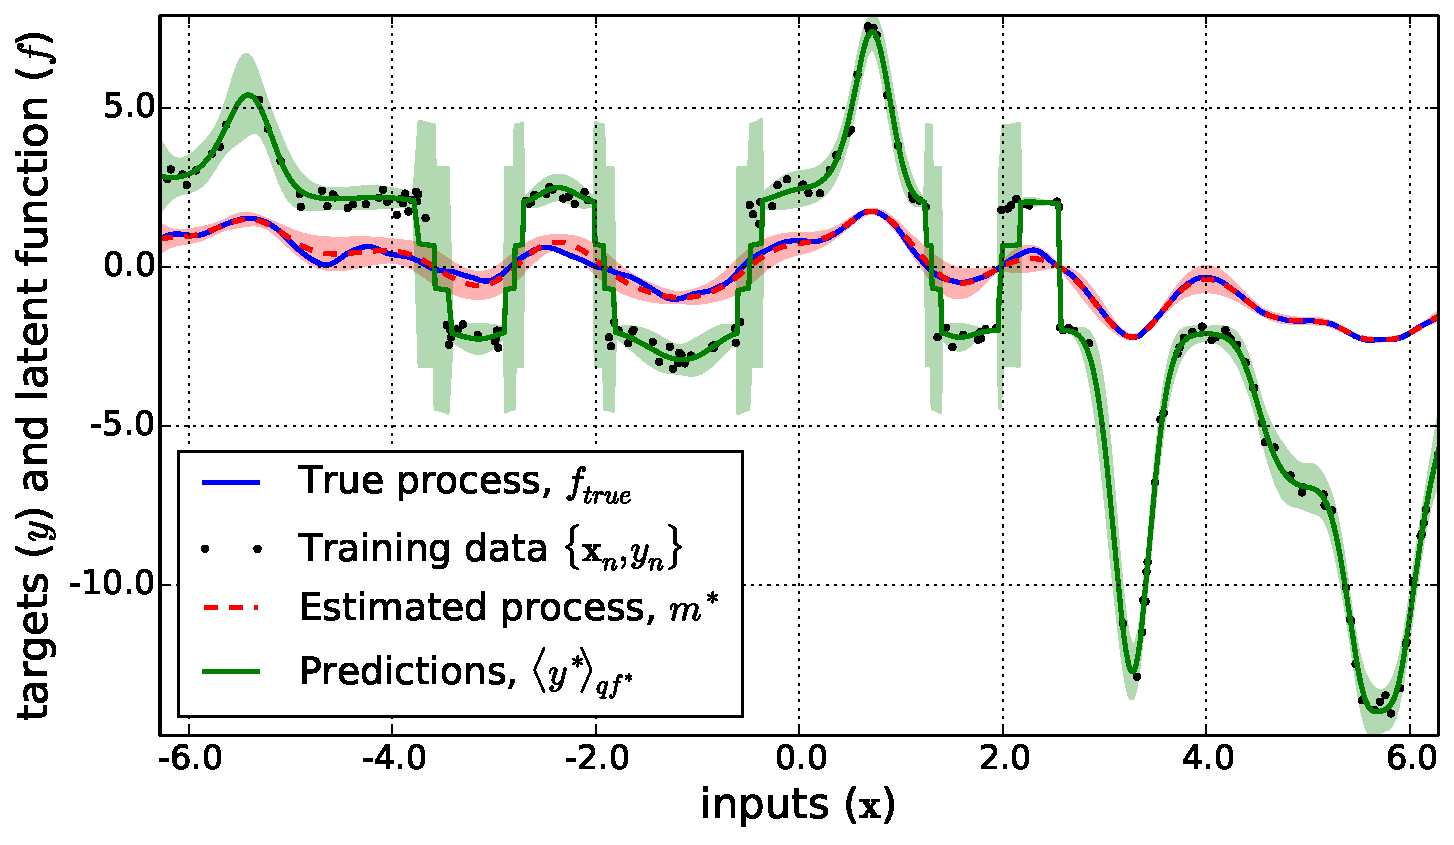
\includegraphics[width=\linewidth]{fig/signdemo}
        \caption{$\nonlin{\lstate} = 2\times\text{sign}\!\brac{\lstate}
            + \lstate^3$}
        \label{sub:sign}
    \end{subfigure}
    \begin{subfigure}[b]{0.5\linewidth}
        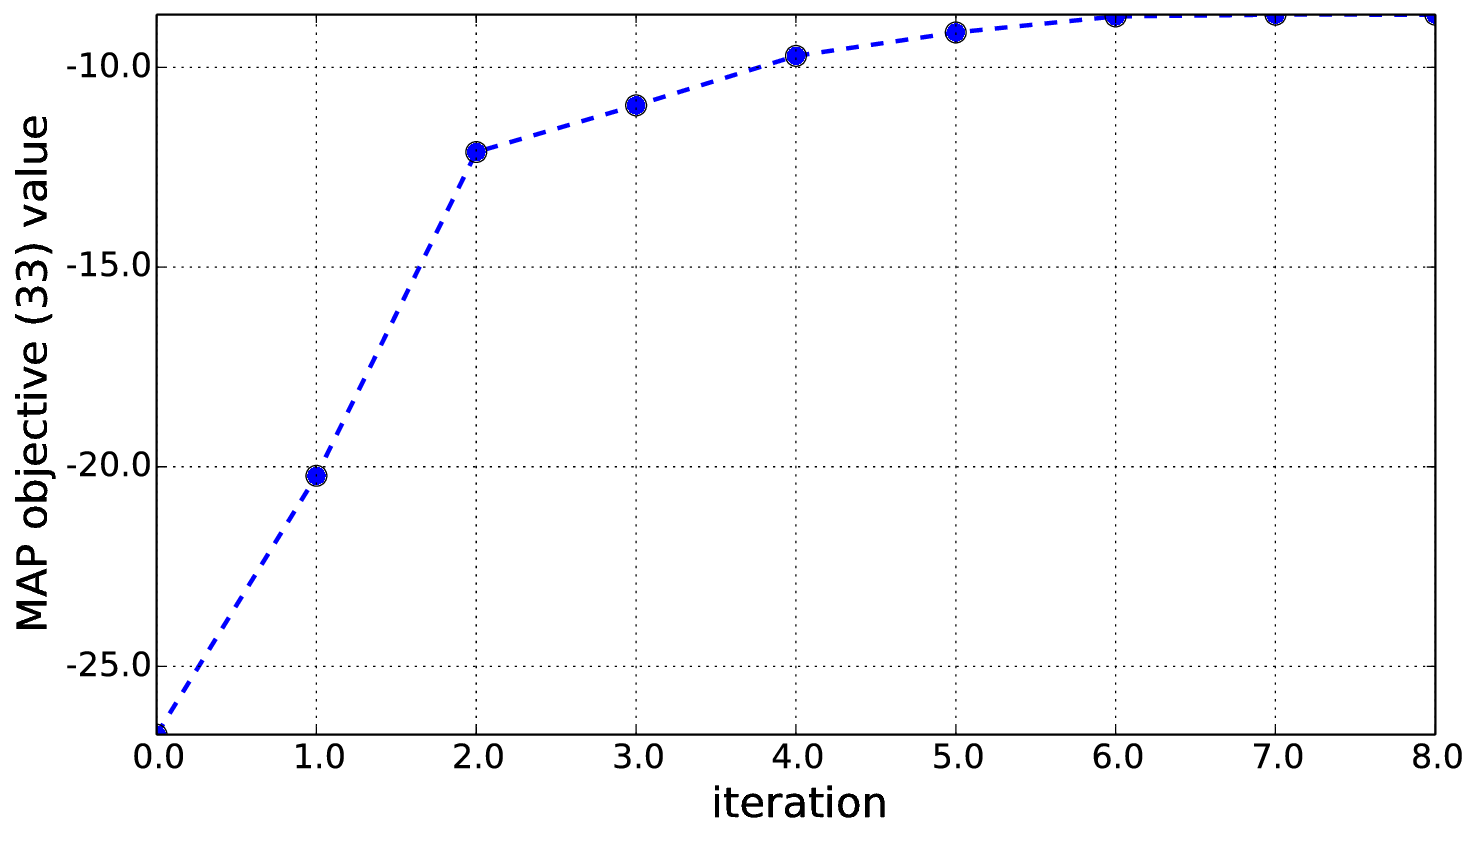
\includegraphics[width=\linewidth]{fig/trace}
        \caption{MAP trace from learning $\pomean$}
        \label{sub:mape}
        \vspace{0.5mm}
    \end{subfigure}

    \caption[]{Learning the UGP with a non-differentiable forward model in
        (\subref{sub:sign}), and a corresponding trace from the MAP objective
        function used to learn $\pomean$ is shown in (\subref{sub:mape}). The
        optimization shown terminated because of a `divergence' condition,
        though the objective function value has still improved.}

    \label{fig:learnex}
\end{figure}

In this experiment we generate `latent' function data from $\lstate \sim
\gaus{\mathbf{0}, \KERNL}$ where a Mat\'ern $\frac{5}{2}$ kernel function is
used with amplitude $\sigma_{m52} = 0.8$, length scale $l_{m52} = 0.6$ and
$\inobs \in \real{}$ are uniformly spaced between $[-2\pi, 2\pi]$ to build
$\KERNL$. Observations used to test and train the GPs are then generated as
$\obs = \nonlin{\lstate} + \epsilon$ where $\epsilon \sim \gaus{0, 0.2^2}$.
1000 points are generated in this way, and we use 5-fold cross validation to
train (200 points) and test (800 points) the GPs. We use standardized mean
squared error (SMSE) to test the predictions with the held out data in both the
latent and observed spaces. We also use  average negative log predictive
density (NLPD) on the latent test data, which is calculated as
$-\frac{1}{N\test} \sum_{n} \log \gausC{\lstates_n\test}{\pomeans_n\test,
    \pocovs_n\test}$. All  GP methods use Mat\'ern $\frac{5}{2}$ covariance
functions with the hyperparameters and $\lvar$ initialized at 1.0 and
lower-bounded at 0.1 (and 0.01 for~$\lvar$).

\autoref{tab:toy} shows results for multiple differentiable forward models,
$\nonlin{\cdot}$. We test the EGP and UGP against the model in \cite{Opper2009}
-- which uses 10,000 samples to evaluate the one dimensional expectations.
Although this number of samples may seem excessive for these simple problems,
our goal here is to have a competitive baseline algorithm. We also test against
normal GP regression for a linear forward model, $\nonlin{\lstate} = \lstate$.
In \autoref{fig:learnex} we show the results of the UGP using a forward model
for which no derivative exists at the zero crossing points, as well as an
objective function trace for learning the posterior mean. We use quadrature for
the predictions in observation space in \autoref{tab:toy} and the unscented
transform, Equation \eqref{eq:slpred}, for the predictions in
\autoref{fig:learnex}. Interestingly, there is almost no difference in
performance between the EGP and UGP, even though the EGP has access to the
derivatives of the forward models and the UGP does not.  Both the UGP and EGP
consistently outperformed \cite{Opper2009} in terms of NLPD and  SMSE, apart
from the $\tanh$ experiment for inversion. In this experiment, the UGP had the
best performance but the EGP was outperformed by \cite{Opper2009}.

%We also found that the method in \cite{Opper2009} would suffer from numerical
%problems  on the non-differentiable forward model in \autoref{fig:learnex}.
%This agrees with the authors who state that their algorithm requires smooth
%likelihood models.


\subsection{Binary Handwritten Digit Classification}

For this experiment we evaluate the EGP and UGP on a classification task. We
are just interested in a probabilistic prediction of class labels, and not the
values of the latent function. We use the USPS handwritten digits dataset with
the task of distinguishing between `3' and `5' -- this is the same experiment
from \cite[\S 3.7.3]{Rasmussen2006}. A logistic sigmoid is used as the forward
model, $\nonlin{\cdot}$, in our algorithms. We test against Laplace,
expectation propagation and variational Bayes logistic GP classifiers (from the
GPML Matlab toolbox \cite{Rasmussen2006}), a support vector machine (SVM) with
a radial basis kernel function (and probabilistic outputs \cite{Platt1999}),
and logistic regression (both from the scikit-learn python library
\cite{scikit-learn}). A squared exponential kernel with amplitude
$\sigma_\text{se}$ and length scale $l_\text{se}$ is used for the GPs in this
experiment. We initialize these hyperparameters at $1.0$, and put a lower bound
of $0.1$ on them. We initialize $\lvar$ and place a lower bound at $10^{-14}$
for the EGP and UGP (the optimized values are near or at this value). The
hyperparameters for the SVM are learned using grid search with three-fold cross
validation. 
%
%of a Bernoulli distribution, $-\frac{1}{N\test} \sum_n \log
%\bernC{\obss_n\test}{\pi\test_n}$ where $\pi\test_n =
%\expec{}{\prob{\obss\test_n = 1}}$ is the probabilistic output of the
%classifier.  as the percentage of incorrectly misclassified labels in the test
%set (once the probabilistic outputs have been thresholded at $0.5$). 

The results are summarized in \autoref{tab:class}, where we report the average
Bernoulli negative log-probability (NLP), the error rate and the learned
hyperparameter values for the GPs. Surprisingly, the UGP outperforms the other
classifiers on this dataset, despite the other classifiers being specifically
formulated for this task. 
%However, we find that our algorithms do get stuck in
%local minima for some large initial values of $\lvar$, e.g.~$1.0$.

\begin{table}[tb]
    \centering

    \caption[]{Classification performance on the USPS handwritten-digits
        dataset for numbers `3' and `5'. Lower values of the negative log
        probability (NLP) and error rate indicate better performance. The
        learned signal variance $\!\brac{\sigma^{2}_\text{se}}$ and length
        scale $\!\brac{l_\text{se}}$ are also shown for consistency with
        \cite[\S 3.7.3]{Rasmussen2006}.}

    \footnotesize
    \begin{tabular}{r| c c c c}
        Algorithm & NLP $\obss\test$ & Error rate (\%) 
            & $\log\!\brac{\sigma_\text{se}}$ & $\log\!\brac{l_\text{se}}$ \\
        \toprule
        GP -- Laplace & 0.11528 & 2.9754 & 2.5855 & 2.5823 \\
        GP -- EP & 0.07522 & 2.4580 & 5.2209 & 2.5315 \\
        GP -- VB & 0.10891 & 3.3635 & 0.9045 & 2.0664 \\ 
        SVM (RBF) & 0.08055 & 2.3286 & -- & -- \\
        Logistic Reg. & 0.11995 & 3.6223 & -- & -- \\
        \midrule
        UGP & \textbf{0.07290} & \textbf{1.9405} & 1.5743 & 1.5262 \\
        EGP & 0.08051 & 2.1992 & 2.9134 & 1.7872 \\
        %UGP & 0.06524 & 2.1992 & 1.5140 & 1.4257 \\
        %EGP & 0.12946 & 2.0699 & 3.3068 & 1.7480 \\
        \bottomrule
    \end{tabular}
    \label{tab:class}
\end{table}


\section{Conclusion and Discussion}

We have presented a variational inference framework with linearization for
Gaussian models with nonlinear likelihood functions, which we show can be used
to derive updates for the extended and unscented Kalman filter algorithms, the
iEKF and the iSPKF. We then generalize these results and develop two inference
algorithms for Gaussian processes, the EGP and UGP. The UGP does not use
derivatives of the nonlinear forward model, yet performs as well as the EGP for
inversion and classification problems. 

Our method is similar to the Warped GP (WGP) \cite{snelson2003warped}, however,
we wish to infer the \emph{full} posterior over the latent function $f$. The
goal of the WGP is to infer a transformation of a non-Gaussian process
observation to a space where a GP can be constructed. That is, the WGP is
concerned with inferring an inverse function $g^{-1}(\cdot)$ so the transformed
(latent) function is well modeled by a GP.

As future work we would like to create multi-task EGPs and UGPs. This would
extend their applicability to inversion problems where the forward models have
multiple inputs and outputs, such as inverse kinematics for dynamical systems.
%We also wish to
%further investigate hyperparameter learning to ascertain if there are other
%effective methods of learning the hyperparameters that do not rely upon
%derivatives of the forward model. 

\subsubsection*{Acknowledgments}
{
\small
This research was supported by the Science Industry Endowment Fund (RP 04-174)
Big Data Knowledge Discovery project. We thank F.\ Ramos, L.\ McCalman, 
S.\ O'Callaghan, A.\ Reid and T.\ Nguyen for 
their helpful feedback.
%
NICTA is funded by the Australian Government through the Department of
Communications and the Australian Research Council through the ICT Centre of
Excellence Program.
}

\bibliographystyle{IEEEtran}
\bibliography{nips2014lin}

\end{document}
